\chapter{Methodology}
\label{ch:methodology}

This chapter will address the core contributions of our project.
We present the hardware involved in sensor fusion, describe the data acquisition procedure, then introduce our final solution, by detailing the research and implementation process, as well as design decisions that had to be made along the way.

\section{Hardware}

In this context, hardware refers to the set of sensors that were used for data collection, determined by the existing industrial setup. The solution was designed such that it does not inherently rely on any particular device, yet there is definitely a relationship between hardware capabilities, data quality and final output, so it is crucial to understand the sensors involved in the process.

\begin{figure}
    \centering
    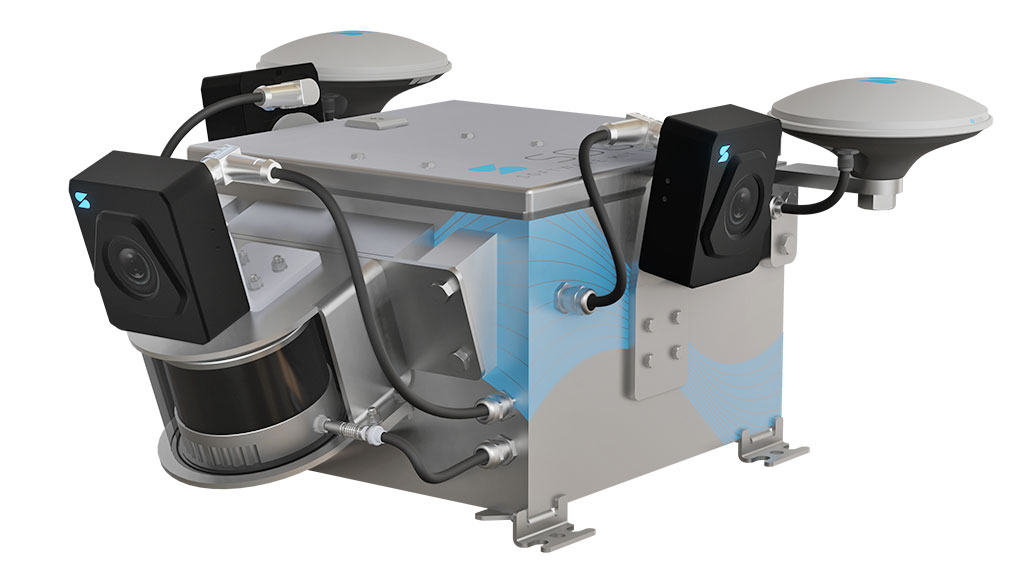
\includegraphics[width=0.6\linewidth]{images/sdx-compact.jpg}
    \caption[SDX-Compact]{The SDX-Compact manufactured by Sodex Innovations GmbH. The set of sensors consists of a 3D LiDAR scanner, three RGB cameras and a high-accuracy positioning system. Image source: \href{https://fieldwork.ch/de/produkte/geopositioning/mobile-datenerfassung/sdx-compact}{Fieldwork}}
    \label{fig:sdx-compact}
\end{figure}

\subsection{LiDAR Sensor}

The SDX-Compact is equipped with a Pandar XT32 \cite{hesai_xt16_32_32m} LiDAR sensor, manufactured by Hesai Technology. This is a mechanical rotating LiDAR with a full $360 \degree$ horizontal field of view and 32 beams distributed vertically, at $1 \degree$ resolution. Horizontal resolution depends on the desired output frequency. With our settings, the sensor produces 10 complete scans per second, resulting in a horizontal resolution of $0.18 \degree$.  The maximum operational range is 120m, but this decreases to 50m for low-reflectivity targets. The official specifications state a typical accuracy of $\pm 1$cm, with precision $\pm 0.5$cm, in a static environment. For each beam, the strongest return is processed, leading to 640,000 points being generated per second. The high output bandwidth is handled by an Ethernet connection, over which points are sent as \acrshort{udp} packets. The sensor also supports \acrshort{ptp} synchronisation, essential for high-quality sensor fusion.

\subsection{GNSS/INS receiver}

Another component of the sensor stack is the Septentrio AsteRx SBi3 Pro+ GNSS/INS receiver \cite{Septentrio_AsteRx_SBi3_Pro+}, which provides global positioning and orientation data at a rate of 100Hz. Internally, this relies on two distinct mechanisms.

The localization information comes from a dual antenna GNSS module compatible with several GNSS consellations (e.g. \acrshort{gps}, \acrshort{glonass}, Galileo), to ensure optimal worldwide coverage. In standalone mode, the advertised typical accuracy is 1m, but the receiver also acts as an NTRIP (a protocol for differential GPS) client, gathering correction information, in order to achieve centimeter-level accuracy.

An \acrfull{imu} module records acceleration data and provides the remaining orientation angles (roll, pitch, yaw) to compute the complete pose, in 6 \acrfull{dof}. This is integrated with the absolute GNSS measurements using the patented FUSE+ technology \cite{Septentrio_FUSE_Sensor_Fusion}, resulting in an orientation error below  $\text{5-10}\degree$.

Like any system reliant on satellite communication, this will suffer significantly in situations where the signal propagation is disturbed (heavy clouds, ``urban canyons'', thick vegetation, spoofing), even leading to loss of \emph{\gls{gnssfix}}.

\subsection{RGB Cameras}

\section{Data acquisition}

\section{Solution architecture}






